% Created by tikzDevice version 0.10.1 on 2018-01-16 22:08:38
% !TEX encoding = UTF-8 Unicode
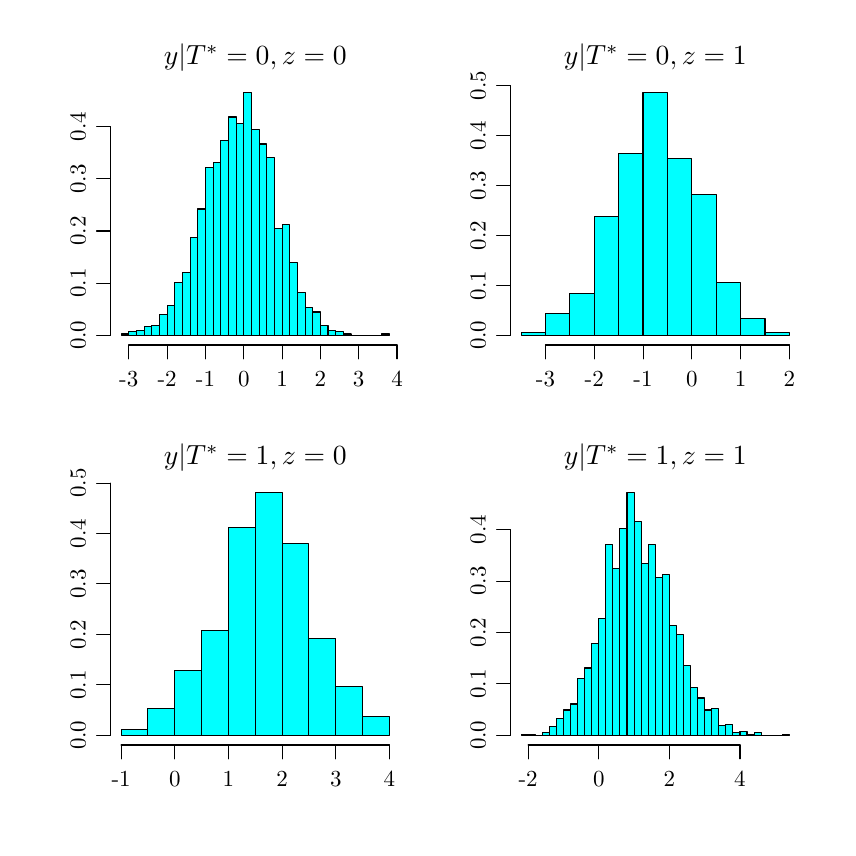
\begin{tikzpicture}[x=1pt,y=1pt]
\definecolor{fillColor}{RGB}{255,255,255}
\path[use as bounding box,fill=fillColor,fill opacity=0.00] (0,0) rectangle (289.08,289.08);
\begin{scope}
\path[clip] (  0.00,  0.00) rectangle (289.08,289.08);
\definecolor{drawColor}{RGB}{0,0,0}

\path[draw=drawColor,line width= 0.4pt,line join=round,line cap=round] ( 36.53,174.42) -- (133.47,174.42);

\path[draw=drawColor,line width= 0.4pt,line join=round,line cap=round] ( 36.53,174.42) -- ( 36.53,169.44);

\path[draw=drawColor,line width= 0.4pt,line join=round,line cap=round] ( 50.38,174.42) -- ( 50.38,169.44);

\path[draw=drawColor,line width= 0.4pt,line join=round,line cap=round] ( 64.23,174.42) -- ( 64.23,169.44);

\path[draw=drawColor,line width= 0.4pt,line join=round,line cap=round] ( 78.08,174.42) -- ( 78.08,169.44);

\path[draw=drawColor,line width= 0.4pt,line join=round,line cap=round] ( 91.93,174.42) -- ( 91.93,169.44);

\path[draw=drawColor,line width= 0.4pt,line join=round,line cap=round] (105.78,174.42) -- (105.78,169.44);

\path[draw=drawColor,line width= 0.4pt,line join=round,line cap=round] (119.63,174.42) -- (119.63,169.44);

\path[draw=drawColor,line width= 0.4pt,line join=round,line cap=round] (133.47,174.42) -- (133.47,169.44);

\node[text=drawColor,anchor=base,inner sep=0pt, outer sep=0pt, scale=  0.83] at ( 36.53,159.48) {-3};

\node[text=drawColor,anchor=base,inner sep=0pt, outer sep=0pt, scale=  0.83] at ( 50.38,159.48) {-2};

\node[text=drawColor,anchor=base,inner sep=0pt, outer sep=0pt, scale=  0.83] at ( 64.23,159.48) {-1};

\node[text=drawColor,anchor=base,inner sep=0pt, outer sep=0pt, scale=  0.83] at ( 78.08,159.48) {0};

\node[text=drawColor,anchor=base,inner sep=0pt, outer sep=0pt, scale=  0.83] at ( 91.93,159.48) {1};

\node[text=drawColor,anchor=base,inner sep=0pt, outer sep=0pt, scale=  0.83] at (105.78,159.48) {2};

\node[text=drawColor,anchor=base,inner sep=0pt, outer sep=0pt, scale=  0.83] at (119.63,159.48) {3};

\node[text=drawColor,anchor=base,inner sep=0pt, outer sep=0pt, scale=  0.83] at (133.47,159.48) {4};

\path[draw=drawColor,line width= 0.4pt,line join=round,line cap=round] ( 29.88,177.93) -- ( 29.88,253.28);

\path[draw=drawColor,line width= 0.4pt,line join=round,line cap=round] ( 29.88,177.93) -- ( 24.90,177.93);

\path[draw=drawColor,line width= 0.4pt,line join=round,line cap=round] ( 29.88,196.77) -- ( 24.90,196.77);

\path[draw=drawColor,line width= 0.4pt,line join=round,line cap=round] ( 29.88,215.61) -- ( 24.90,215.61);

\path[draw=drawColor,line width= 0.4pt,line join=round,line cap=round] ( 29.88,234.44) -- ( 24.90,234.44);

\path[draw=drawColor,line width= 0.4pt,line join=round,line cap=round] ( 29.88,253.28) -- ( 24.90,253.28);

\node[text=drawColor,rotate= 90.00,anchor=base,inner sep=0pt, outer sep=0pt, scale=  0.83] at ( 20.92,177.93) {0.0};

\node[text=drawColor,rotate= 90.00,anchor=base,inner sep=0pt, outer sep=0pt, scale=  0.83] at ( 20.92,196.77) {0.1};

\node[text=drawColor,rotate= 90.00,anchor=base,inner sep=0pt, outer sep=0pt, scale=  0.83] at ( 20.92,215.61) {0.2};

\node[text=drawColor,rotate= 90.00,anchor=base,inner sep=0pt, outer sep=0pt, scale=  0.83] at ( 20.92,234.44) {0.3};

\node[text=drawColor,rotate= 90.00,anchor=base,inner sep=0pt, outer sep=0pt, scale=  0.83] at ( 20.92,253.28) {0.4};
\end{scope}
\begin{scope}
\path[clip] (  0.00,144.54) rectangle (144.54,289.08);
\definecolor{drawColor}{RGB}{0,0,0}

\node[text=drawColor,anchor=base,inner sep=0pt, outer sep=0pt, scale=  1.00] at ( 82.23,275.68) {\bfseries $y|T^*=0,z=0$};
\end{scope}
\begin{scope}
\path[clip] ( 29.88,174.42) rectangle (134.58,269.16);
\definecolor{drawColor}{RGB}{0,0,0}
\definecolor{fillColor}{RGB}{0,255,255}

\path[draw=drawColor,line width= 0.4pt,line join=round,line cap=round,fill=fillColor] ( 33.76,177.93) rectangle ( 36.53,178.37);

\path[draw=drawColor,line width= 0.4pt,line join=round,line cap=round,fill=fillColor] ( 36.53,177.93) rectangle ( 39.30,179.26);

\path[draw=drawColor,line width= 0.4pt,line join=round,line cap=round,fill=fillColor] ( 39.30,177.93) rectangle ( 42.07,179.70);

\path[draw=drawColor,line width= 0.4pt,line join=round,line cap=round,fill=fillColor] ( 42.07,177.93) rectangle ( 44.84,181.03);

\path[draw=drawColor,line width= 0.4pt,line join=round,line cap=round,fill=fillColor] ( 44.84,177.93) rectangle ( 47.61,181.47);

\path[draw=drawColor,line width= 0.4pt,line join=round,line cap=round,fill=fillColor] ( 47.61,177.93) rectangle ( 50.38,185.46);

\path[draw=drawColor,line width= 0.4pt,line join=round,line cap=round,fill=fillColor] ( 50.38,177.93) rectangle ( 53.15,188.56);

\path[draw=drawColor,line width= 0.4pt,line join=round,line cap=round,fill=fillColor] ( 53.15,177.93) rectangle ( 55.92,196.98);

\path[draw=drawColor,line width= 0.4pt,line join=round,line cap=round,fill=fillColor] ( 55.92,177.93) rectangle ( 58.69,200.52);

\path[draw=drawColor,line width= 0.4pt,line join=round,line cap=round,fill=fillColor] ( 58.69,177.93) rectangle ( 61.46,213.37);

\path[draw=drawColor,line width= 0.4pt,line join=round,line cap=round,fill=fillColor] ( 61.46,177.93) rectangle ( 64.23,223.56);

\path[draw=drawColor,line width= 0.4pt,line join=round,line cap=round,fill=fillColor] ( 64.23,177.93) rectangle ( 67.00,238.63);

\path[draw=drawColor,line width= 0.4pt,line join=round,line cap=round,fill=fillColor] ( 67.00,177.93) rectangle ( 69.77,240.40);

\path[draw=drawColor,line width= 0.4pt,line join=round,line cap=round,fill=fillColor] ( 69.77,177.93) rectangle ( 72.54,248.37);

\path[draw=drawColor,line width= 0.4pt,line join=round,line cap=round,fill=fillColor] ( 72.54,177.93) rectangle ( 75.31,256.79);

\path[draw=drawColor,line width= 0.4pt,line join=round,line cap=round,fill=fillColor] ( 75.31,177.93) rectangle ( 78.08,254.58);

\path[draw=drawColor,line width= 0.4pt,line join=round,line cap=round,fill=fillColor] ( 78.08,177.93) rectangle ( 80.85,265.65);

\path[draw=drawColor,line width= 0.4pt,line join=round,line cap=round,fill=fillColor] ( 80.85,177.93) rectangle ( 83.61,252.36);

\path[draw=drawColor,line width= 0.4pt,line join=round,line cap=round,fill=fillColor] ( 83.61,177.93) rectangle ( 86.38,247.04);

\path[draw=drawColor,line width= 0.4pt,line join=round,line cap=round,fill=fillColor] ( 86.38,177.93) rectangle ( 89.15,242.17);

\path[draw=drawColor,line width= 0.4pt,line join=round,line cap=round,fill=fillColor] ( 89.15,177.93) rectangle ( 91.92,216.47);

\path[draw=drawColor,line width= 0.4pt,line join=round,line cap=round,fill=fillColor] ( 91.92,177.93) rectangle ( 94.69,217.80);

\path[draw=drawColor,line width= 0.4pt,line join=round,line cap=round,fill=fillColor] ( 94.69,177.93) rectangle ( 97.46,204.07);

\path[draw=drawColor,line width= 0.4pt,line join=round,line cap=round,fill=fillColor] ( 97.46,177.93) rectangle (100.23,193.44);

\path[draw=drawColor,line width= 0.4pt,line join=round,line cap=round,fill=fillColor] (100.23,177.93) rectangle (103.00,188.12);

\path[draw=drawColor,line width= 0.4pt,line join=round,line cap=round,fill=fillColor] (103.00,177.93) rectangle (105.77,186.35);

\path[draw=drawColor,line width= 0.4pt,line join=round,line cap=round,fill=fillColor] (105.77,177.93) rectangle (108.54,181.47);

\path[draw=drawColor,line width= 0.4pt,line join=round,line cap=round,fill=fillColor] (108.54,177.93) rectangle (111.31,179.70);

\path[draw=drawColor,line width= 0.4pt,line join=round,line cap=round,fill=fillColor] (111.31,177.93) rectangle (114.08,179.26);

\path[draw=drawColor,line width= 0.4pt,line join=round,line cap=round,fill=fillColor] (114.08,177.93) rectangle (116.85,178.37);

\path[draw=drawColor,line width= 0.4pt,line join=round,line cap=round,fill=fillColor] (116.85,177.93) rectangle (119.62,177.93);

\path[draw=drawColor,line width= 0.4pt,line join=round,line cap=round,fill=fillColor] (119.62,177.93) rectangle (122.39,177.93);

\path[draw=drawColor,line width= 0.4pt,line join=round,line cap=round,fill=fillColor] (122.39,177.93) rectangle (125.16,177.93);

\path[draw=drawColor,line width= 0.4pt,line join=round,line cap=round,fill=fillColor] (125.16,177.93) rectangle (127.93,177.93);

\path[draw=drawColor,line width= 0.4pt,line join=round,line cap=round,fill=fillColor] (127.93,177.93) rectangle (130.70,178.37);
\end{scope}
\begin{scope}
\path[clip] (  0.00,  0.00) rectangle (289.08,289.08);
\definecolor{drawColor}{RGB}{0,0,0}

\path[draw=drawColor,line width= 0.4pt,line join=round,line cap=round] (187.12,174.42) -- (275.25,174.42);

\path[draw=drawColor,line width= 0.4pt,line join=round,line cap=round] (187.12,174.42) -- (187.12,169.44);

\path[draw=drawColor,line width= 0.4pt,line join=round,line cap=round] (204.75,174.42) -- (204.75,169.44);

\path[draw=drawColor,line width= 0.4pt,line join=round,line cap=round] (222.37,174.42) -- (222.37,169.44);

\path[draw=drawColor,line width= 0.4pt,line join=round,line cap=round] (240.00,174.42) -- (240.00,169.44);

\path[draw=drawColor,line width= 0.4pt,line join=round,line cap=round] (257.62,174.42) -- (257.62,169.44);

\path[draw=drawColor,line width= 0.4pt,line join=round,line cap=round] (275.25,174.42) -- (275.25,169.44);

\node[text=drawColor,anchor=base,inner sep=0pt, outer sep=0pt, scale=  0.83] at (187.12,159.48) {-3};

\node[text=drawColor,anchor=base,inner sep=0pt, outer sep=0pt, scale=  0.83] at (204.75,159.48) {-2};

\node[text=drawColor,anchor=base,inner sep=0pt, outer sep=0pt, scale=  0.83] at (222.37,159.48) {-1};

\node[text=drawColor,anchor=base,inner sep=0pt, outer sep=0pt, scale=  0.83] at (240.00,159.48) {0};

\node[text=drawColor,anchor=base,inner sep=0pt, outer sep=0pt, scale=  0.83] at (257.62,159.48) {1};

\node[text=drawColor,anchor=base,inner sep=0pt, outer sep=0pt, scale=  0.83] at (275.25,159.48) {2};

\path[draw=drawColor,line width= 0.4pt,line join=round,line cap=round] (174.42,177.93) -- (174.42,268.14);

\path[draw=drawColor,line width= 0.4pt,line join=round,line cap=round] (174.42,177.93) -- (169.44,177.93);

\path[draw=drawColor,line width= 0.4pt,line join=round,line cap=round] (174.42,195.97) -- (169.44,195.97);

\path[draw=drawColor,line width= 0.4pt,line join=round,line cap=round] (174.42,214.01) -- (169.44,214.01);

\path[draw=drawColor,line width= 0.4pt,line join=round,line cap=round] (174.42,232.06) -- (169.44,232.06);

\path[draw=drawColor,line width= 0.4pt,line join=round,line cap=round] (174.42,250.10) -- (169.44,250.10);

\path[draw=drawColor,line width= 0.4pt,line join=round,line cap=round] (174.42,268.14) -- (169.44,268.14);

\node[text=drawColor,rotate= 90.00,anchor=base,inner sep=0pt, outer sep=0pt, scale=  0.83] at (165.46,177.93) {0.0};

\node[text=drawColor,rotate= 90.00,anchor=base,inner sep=0pt, outer sep=0pt, scale=  0.83] at (165.46,195.97) {0.1};

\node[text=drawColor,rotate= 90.00,anchor=base,inner sep=0pt, outer sep=0pt, scale=  0.83] at (165.46,214.01) {0.2};

\node[text=drawColor,rotate= 90.00,anchor=base,inner sep=0pt, outer sep=0pt, scale=  0.83] at (165.46,232.06) {0.3};

\node[text=drawColor,rotate= 90.00,anchor=base,inner sep=0pt, outer sep=0pt, scale=  0.83] at (165.46,250.10) {0.4};

\node[text=drawColor,rotate= 90.00,anchor=base,inner sep=0pt, outer sep=0pt, scale=  0.83] at (165.46,268.14) {0.5};
\end{scope}
\begin{scope}
\path[clip] (144.54,144.54) rectangle (289.08,289.08);
\definecolor{drawColor}{RGB}{0,0,0}

\node[text=drawColor,anchor=base,inner sep=0pt, outer sep=0pt, scale=  1.00] at (226.77,275.68) {\bfseries $y|T^*=0,z=1$};
\end{scope}
\begin{scope}
\path[clip] (174.42,174.42) rectangle (279.12,269.16);
\definecolor{drawColor}{RGB}{0,0,0}
\definecolor{fillColor}{RGB}{0,255,255}

\path[draw=drawColor,line width= 0.4pt,line join=round,line cap=round,fill=fillColor] (178.30,177.93) rectangle (187.11,178.93);

\path[draw=drawColor,line width= 0.4pt,line join=round,line cap=round,fill=fillColor] (187.11,177.93) rectangle (195.92,185.90);

\path[draw=drawColor,line width= 0.4pt,line join=round,line cap=round,fill=fillColor] (195.92,177.93) rectangle (204.74,192.88);

\path[draw=drawColor,line width= 0.4pt,line join=round,line cap=round,fill=fillColor] (204.74,177.93) rectangle (213.55,220.79);

\path[draw=drawColor,line width= 0.4pt,line join=round,line cap=round,fill=fillColor] (213.55,177.93) rectangle (222.36,243.72);

\path[draw=drawColor,line width= 0.4pt,line join=round,line cap=round,fill=fillColor] (222.36,177.93) rectangle (231.18,265.65);

\path[draw=drawColor,line width= 0.4pt,line join=round,line cap=round,fill=fillColor] (231.18,177.93) rectangle (239.99,241.73);

\path[draw=drawColor,line width= 0.4pt,line join=round,line cap=round,fill=fillColor] (239.99,177.93) rectangle (248.80,228.77);

\path[draw=drawColor,line width= 0.4pt,line join=round,line cap=round,fill=fillColor] (248.80,177.93) rectangle (257.62,196.87);

\path[draw=drawColor,line width= 0.4pt,line join=round,line cap=round,fill=fillColor] (257.62,177.93) rectangle (266.43,183.91);

\path[draw=drawColor,line width= 0.4pt,line join=round,line cap=round,fill=fillColor] (266.43,177.93) rectangle (275.24,178.93);
\end{scope}
\begin{scope}
\path[clip] (  0.00,  0.00) rectangle (289.08,289.08);
\definecolor{drawColor}{RGB}{0,0,0}

\path[draw=drawColor,line width= 0.4pt,line join=round,line cap=round] ( 33.77, 29.88) -- (130.71, 29.88);

\path[draw=drawColor,line width= 0.4pt,line join=round,line cap=round] ( 33.77, 29.88) -- ( 33.77, 24.90);

\path[draw=drawColor,line width= 0.4pt,line join=round,line cap=round] ( 53.16, 29.88) -- ( 53.16, 24.90);

\path[draw=drawColor,line width= 0.4pt,line join=round,line cap=round] ( 72.55, 29.88) -- ( 72.55, 24.90);

\path[draw=drawColor,line width= 0.4pt,line join=round,line cap=round] ( 91.93, 29.88) -- ( 91.93, 24.90);

\path[draw=drawColor,line width= 0.4pt,line join=round,line cap=round] (111.32, 29.88) -- (111.32, 24.90);

\path[draw=drawColor,line width= 0.4pt,line join=round,line cap=round] (130.71, 29.88) -- (130.71, 24.90);

\node[text=drawColor,anchor=base,inner sep=0pt, outer sep=0pt, scale=  0.83] at ( 33.77, 14.94) {-1};

\node[text=drawColor,anchor=base,inner sep=0pt, outer sep=0pt, scale=  0.83] at ( 53.16, 14.94) {0};

\node[text=drawColor,anchor=base,inner sep=0pt, outer sep=0pt, scale=  0.83] at ( 72.55, 14.94) {1};

\node[text=drawColor,anchor=base,inner sep=0pt, outer sep=0pt, scale=  0.83] at ( 91.93, 14.94) {2};

\node[text=drawColor,anchor=base,inner sep=0pt, outer sep=0pt, scale=  0.83] at (111.32, 14.94) {3};

\node[text=drawColor,anchor=base,inner sep=0pt, outer sep=0pt, scale=  0.83] at (130.71, 14.94) {4};

\path[draw=drawColor,line width= 0.4pt,line join=round,line cap=round] ( 29.88, 33.39) -- ( 29.88,124.52);

\path[draw=drawColor,line width= 0.4pt,line join=round,line cap=round] ( 29.88, 33.39) -- ( 24.90, 33.39);

\path[draw=drawColor,line width= 0.4pt,line join=round,line cap=round] ( 29.88, 51.62) -- ( 24.90, 51.62);

\path[draw=drawColor,line width= 0.4pt,line join=round,line cap=round] ( 29.88, 69.84) -- ( 24.90, 69.84);

\path[draw=drawColor,line width= 0.4pt,line join=round,line cap=round] ( 29.88, 88.07) -- ( 24.90, 88.07);

\path[draw=drawColor,line width= 0.4pt,line join=round,line cap=round] ( 29.88,106.30) -- ( 24.90,106.30);

\path[draw=drawColor,line width= 0.4pt,line join=round,line cap=round] ( 29.88,124.52) -- ( 24.90,124.52);

\node[text=drawColor,rotate= 90.00,anchor=base,inner sep=0pt, outer sep=0pt, scale=  0.83] at ( 20.92, 33.39) {0.0};

\node[text=drawColor,rotate= 90.00,anchor=base,inner sep=0pt, outer sep=0pt, scale=  0.83] at ( 20.92, 51.62) {0.1};

\node[text=drawColor,rotate= 90.00,anchor=base,inner sep=0pt, outer sep=0pt, scale=  0.83] at ( 20.92, 69.84) {0.2};

\node[text=drawColor,rotate= 90.00,anchor=base,inner sep=0pt, outer sep=0pt, scale=  0.83] at ( 20.92, 88.07) {0.3};

\node[text=drawColor,rotate= 90.00,anchor=base,inner sep=0pt, outer sep=0pt, scale=  0.83] at ( 20.92,106.30) {0.4};

\node[text=drawColor,rotate= 90.00,anchor=base,inner sep=0pt, outer sep=0pt, scale=  0.83] at ( 20.92,124.52) {0.5};
\end{scope}
\begin{scope}
\path[clip] (  0.00,  0.00) rectangle (144.54,144.54);
\definecolor{drawColor}{RGB}{0,0,0}

\node[text=drawColor,anchor=base,inner sep=0pt, outer sep=0pt, scale=  1.00] at ( 82.23,131.14) {\bfseries $y|T^*=1,z=0$};
\end{scope}
\begin{scope}
\path[clip] ( 29.88, 29.88) rectangle (134.58,124.62);
\definecolor{drawColor}{RGB}{0,0,0}
\definecolor{fillColor}{RGB}{0,255,255}

\path[draw=drawColor,line width= 0.4pt,line join=round,line cap=round,fill=fillColor] ( 33.76, 33.39) rectangle ( 43.45, 35.34);

\path[draw=drawColor,line width= 0.4pt,line join=round,line cap=round,fill=fillColor] ( 43.45, 33.39) rectangle ( 53.15, 43.14);

\path[draw=drawColor,line width= 0.4pt,line join=round,line cap=round,fill=fillColor] ( 53.15, 33.39) rectangle ( 62.84, 56.78);

\path[draw=drawColor,line width= 0.4pt,line join=round,line cap=round,fill=fillColor] ( 62.84, 33.39) rectangle ( 72.54, 71.40);

\path[draw=drawColor,line width= 0.4pt,line join=round,line cap=round,fill=fillColor] ( 72.54, 33.39) rectangle ( 82.23,108.44);

\path[draw=drawColor,line width= 0.4pt,line join=round,line cap=round,fill=fillColor] ( 82.23, 33.39) rectangle ( 91.92,121.11);

\path[draw=drawColor,line width= 0.4pt,line join=round,line cap=round,fill=fillColor] ( 91.92, 33.39) rectangle (101.62,102.59);

\path[draw=drawColor,line width= 0.4pt,line join=round,line cap=round,fill=fillColor] (101.62, 33.39) rectangle (111.31, 68.48);

\path[draw=drawColor,line width= 0.4pt,line join=round,line cap=round,fill=fillColor] (111.31, 33.39) rectangle (121.01, 50.93);

\path[draw=drawColor,line width= 0.4pt,line join=round,line cap=round,fill=fillColor] (121.01, 33.39) rectangle (130.70, 40.21);
\end{scope}
\begin{scope}
\path[clip] (  0.00,  0.00) rectangle (289.08,289.08);
\definecolor{drawColor}{RGB}{0,0,0}

\path[draw=drawColor,line width= 0.4pt,line join=round,line cap=round] (180.85, 29.88) -- (257.39, 29.88);

\path[draw=drawColor,line width= 0.4pt,line join=round,line cap=round] (180.85, 29.88) -- (180.85, 24.90);

\path[draw=drawColor,line width= 0.4pt,line join=round,line cap=round] (206.36, 29.88) -- (206.36, 24.90);

\path[draw=drawColor,line width= 0.4pt,line join=round,line cap=round] (231.87, 29.88) -- (231.87, 24.90);

\path[draw=drawColor,line width= 0.4pt,line join=round,line cap=round] (257.39, 29.88) -- (257.39, 24.90);

\node[text=drawColor,anchor=base,inner sep=0pt, outer sep=0pt, scale=  0.83] at (180.85, 14.94) {-2};

\node[text=drawColor,anchor=base,inner sep=0pt, outer sep=0pt, scale=  0.83] at (206.36, 14.94) {0};

\node[text=drawColor,anchor=base,inner sep=0pt, outer sep=0pt, scale=  0.83] at (231.87, 14.94) {2};

\node[text=drawColor,anchor=base,inner sep=0pt, outer sep=0pt, scale=  0.83] at (257.39, 14.94) {4};

\path[draw=drawColor,line width= 0.4pt,line join=round,line cap=round] (174.42, 33.39) -- (174.42,107.67);

\path[draw=drawColor,line width= 0.4pt,line join=round,line cap=round] (174.42, 33.39) -- (169.44, 33.39);

\path[draw=drawColor,line width= 0.4pt,line join=round,line cap=round] (174.42, 51.96) -- (169.44, 51.96);

\path[draw=drawColor,line width= 0.4pt,line join=round,line cap=round] (174.42, 70.53) -- (169.44, 70.53);

\path[draw=drawColor,line width= 0.4pt,line join=round,line cap=round] (174.42, 89.10) -- (169.44, 89.10);

\path[draw=drawColor,line width= 0.4pt,line join=round,line cap=round] (174.42,107.67) -- (169.44,107.67);

\node[text=drawColor,rotate= 90.00,anchor=base,inner sep=0pt, outer sep=0pt, scale=  0.83] at (165.46, 33.39) {0.0};

\node[text=drawColor,rotate= 90.00,anchor=base,inner sep=0pt, outer sep=0pt, scale=  0.83] at (165.46, 51.96) {0.1};

\node[text=drawColor,rotate= 90.00,anchor=base,inner sep=0pt, outer sep=0pt, scale=  0.83] at (165.46, 70.53) {0.2};

\node[text=drawColor,rotate= 90.00,anchor=base,inner sep=0pt, outer sep=0pt, scale=  0.83] at (165.46, 89.10) {0.3};

\node[text=drawColor,rotate= 90.00,anchor=base,inner sep=0pt, outer sep=0pt, scale=  0.83] at (165.46,107.67) {0.4};
\end{scope}
\begin{scope}
\path[clip] (144.54,  0.00) rectangle (289.08,144.54);
\definecolor{drawColor}{RGB}{0,0,0}

\node[text=drawColor,anchor=base,inner sep=0pt, outer sep=0pt, scale=  1.00] at (226.77,131.14) {\bfseries $y|T^*=1,z=1$};
\end{scope}
\begin{scope}
\path[clip] (174.42, 29.88) rectangle (279.12,124.62);
\definecolor{drawColor}{RGB}{0,0,0}
\definecolor{fillColor}{RGB}{0,255,255}

\path[draw=drawColor,line width= 0.4pt,line join=round,line cap=round,fill=fillColor] (178.30, 33.39) rectangle (180.85, 33.82);

\path[draw=drawColor,line width= 0.4pt,line join=round,line cap=round,fill=fillColor] (180.85, 33.39) rectangle (183.40, 33.82);

\path[draw=drawColor,line width= 0.4pt,line join=round,line cap=round,fill=fillColor] (183.40, 33.39) rectangle (185.95, 33.39);

\path[draw=drawColor,line width= 0.4pt,line join=round,line cap=round,fill=fillColor] (185.95, 33.39) rectangle (188.50, 34.26);

\path[draw=drawColor,line width= 0.4pt,line join=round,line cap=round,fill=fillColor] (188.50, 33.39) rectangle (191.05, 36.43);

\path[draw=drawColor,line width= 0.4pt,line join=round,line cap=round,fill=fillColor] (191.05, 33.39) rectangle (193.60, 39.47);

\path[draw=drawColor,line width= 0.4pt,line join=round,line cap=round,fill=fillColor] (193.60, 33.39) rectangle (196.16, 42.51);

\path[draw=drawColor,line width= 0.4pt,line join=round,line cap=round,fill=fillColor] (196.16, 33.39) rectangle (198.71, 44.68);

\path[draw=drawColor,line width= 0.4pt,line join=round,line cap=round,fill=fillColor] (198.71, 33.39) rectangle (201.26, 53.80);

\path[draw=drawColor,line width= 0.4pt,line join=round,line cap=round,fill=fillColor] (201.26, 33.39) rectangle (203.81, 57.71);

\path[draw=drawColor,line width= 0.4pt,line join=round,line cap=round,fill=fillColor] (203.81, 33.39) rectangle (206.36, 66.39);

\path[draw=drawColor,line width= 0.4pt,line join=round,line cap=round,fill=fillColor] (206.36, 33.39) rectangle (208.91, 75.51);

\path[draw=drawColor,line width= 0.4pt,line join=round,line cap=round,fill=fillColor] (208.91, 33.39) rectangle (211.46,102.44);

\path[draw=drawColor,line width= 0.4pt,line join=round,line cap=round,fill=fillColor] (211.46, 33.39) rectangle (214.01, 93.75);

\path[draw=drawColor,line width= 0.4pt,line join=round,line cap=round,fill=fillColor] (214.01, 33.39) rectangle (216.57,108.08);

\path[draw=drawColor,line width= 0.4pt,line join=round,line cap=round,fill=fillColor] (216.57, 33.39) rectangle (219.12,121.11);

\path[draw=drawColor,line width= 0.4pt,line join=round,line cap=round,fill=fillColor] (219.12, 33.39) rectangle (221.67,110.69);

\path[draw=drawColor,line width= 0.4pt,line join=round,line cap=round,fill=fillColor] (221.67, 33.39) rectangle (224.22, 95.49);

\path[draw=drawColor,line width= 0.4pt,line join=round,line cap=round,fill=fillColor] (224.22, 33.39) rectangle (226.77,102.44);

\path[draw=drawColor,line width= 0.4pt,line join=round,line cap=round,fill=fillColor] (226.77, 33.39) rectangle (229.32, 90.28);

\path[draw=drawColor,line width= 0.4pt,line join=round,line cap=round,fill=fillColor] (229.32, 33.39) rectangle (231.87, 91.58);

\path[draw=drawColor,line width= 0.4pt,line join=round,line cap=round,fill=fillColor] (231.87, 33.39) rectangle (234.42, 72.91);

\path[draw=drawColor,line width= 0.4pt,line join=round,line cap=round,fill=fillColor] (234.42, 33.39) rectangle (236.97, 69.87);

\path[draw=drawColor,line width= 0.4pt,line join=round,line cap=round,fill=fillColor] (236.97, 33.39) rectangle (239.53, 58.58);

\path[draw=drawColor,line width= 0.4pt,line join=round,line cap=round,fill=fillColor] (239.53, 33.39) rectangle (242.08, 50.76);

\path[draw=drawColor,line width= 0.4pt,line join=round,line cap=round,fill=fillColor] (242.08, 33.39) rectangle (244.63, 46.85);

\path[draw=drawColor,line width= 0.4pt,line join=round,line cap=round,fill=fillColor] (244.63, 33.39) rectangle (247.18, 42.51);

\path[draw=drawColor,line width= 0.4pt,line join=round,line cap=round,fill=fillColor] (247.18, 33.39) rectangle (249.73, 42.94);

\path[draw=drawColor,line width= 0.4pt,line join=round,line cap=round,fill=fillColor] (249.73, 33.39) rectangle (252.28, 36.86);

\path[draw=drawColor,line width= 0.4pt,line join=round,line cap=round,fill=fillColor] (252.28, 33.39) rectangle (254.83, 37.30);

\path[draw=drawColor,line width= 0.4pt,line join=round,line cap=round,fill=fillColor] (254.83, 33.39) rectangle (257.38, 34.26);

\path[draw=drawColor,line width= 0.4pt,line join=round,line cap=round,fill=fillColor] (257.38, 33.39) rectangle (259.94, 34.69);

\path[draw=drawColor,line width= 0.4pt,line join=round,line cap=round,fill=fillColor] (259.94, 33.39) rectangle (262.49, 33.82);

\path[draw=drawColor,line width= 0.4pt,line join=round,line cap=round,fill=fillColor] (262.49, 33.39) rectangle (265.04, 34.26);

\path[draw=drawColor,line width= 0.4pt,line join=round,line cap=round,fill=fillColor] (265.04, 33.39) rectangle (267.59, 33.39);

\path[draw=drawColor,line width= 0.4pt,line join=round,line cap=round,fill=fillColor] (267.59, 33.39) rectangle (270.14, 33.39);

\path[draw=drawColor,line width= 0.4pt,line join=round,line cap=round,fill=fillColor] (270.14, 33.39) rectangle (272.69, 33.39);

\path[draw=drawColor,line width= 0.4pt,line join=round,line cap=round,fill=fillColor] (272.69, 33.39) rectangle (275.24, 33.82);
\end{scope}
\end{tikzpicture}
